\chapter{Nicht-Unterhalbstetigkeit und Relaxierung}
\textit{Quelle für Definitionen/Sätze dieses Kapitels: \cite{CalcVarJost}[Seite 208 ff.]}\\[0.1cm]
Wir haben in Kapitel 1 gesehen, dass nicht-unterhalbstetige (uhs) Funktionale nicht abstrakt-künstlicher Natur sind, sondern durchaus in der Anwendung immer wieder auftreten. Wir werden uns deshalb ansehen, wie wir mit solchen Fällen umgehen können. Wir werden in Kapitel 3 dann auch auf das Bolza-Beispiel zurückkommen.\\

\pgfsetfillopacity{0.2}\colorbox{defblue}{\begin{minipage}{16cm}{\textcolor{black}{\pgfsetfillopacity{1}}{\label{def2.1}}}
\textbf{Definition 2.1 (Relaxierung):} Betrachte einen topologischen Raum \((X,\tau)\), kurz \(X\) und ein Funktional \(\mathcal{F}:X \to \overline{\mathbb{R}}\). Dann definieren wir die uhs Einhüllende bzw. das relaxierte Funktional (oder einfach nur Relaxierte) \(sc^- \mathcal{F}\) von \(\mathcal{F}\) durch:
\begin{equation}
    (sc^-\mathcal{F})[x] := \sup \{\Phi[x] \, | \, \Phi : X \to \overline{\mathbb{R}} \text{ ist uhs mit }\Phi[y] \le \mathcal{F}[y] \, \forall y \in X\}
\end{equation}
\end{minipage}}

\textbf{Bemerkung:} Die Relaxierte ist die größte uhs Funktion auf \(X\), die \(\le \mathcal{F}\) ist. Dies entnimmt man direkt der Definition und der Tatsache, dass die Relaxierte uhs als Supremum von uhs Funktionalen ist.\\
Warum man genau die uhs Einhüllende wählt, wird dann im Folgevortrag über \(\Gamma-\\\)Konvergenz noch klar.\\

\begin{figure}[!h]
    \centering
    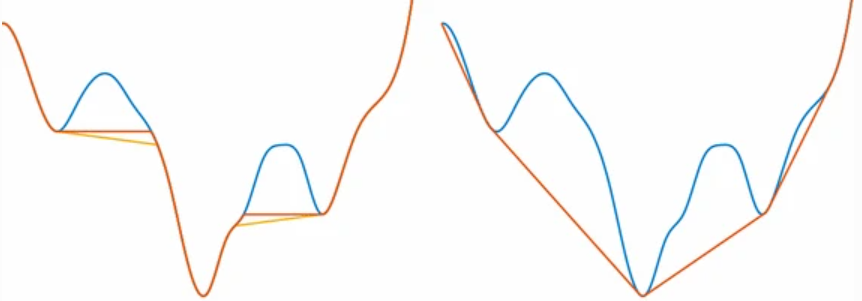
\includegraphics[scale=0.8]{figures/Einhuellende.png}
    \caption{Das Konzept der Einhüllenden: In blau eine gegebene Funktion; quasikonvexe Einhüllende (rot/orange), robust quasikonvexe Einhüllende (gelb) links; konvexe Einhüllende (rot/orange) rechts \cite{ConvexEnvelope}}
    \label{fig:einh}
\end{figure}

Kommen wir nun zurück auf die Ursprungsfrage, wie man im Falle von nicht-\\unterhalbstetigen Funktionalen die Minimierung "reparieren" kann. Der folgende Satz beantwortet diese Frage:\\
\pgfsetfillopacity{0.2}\colorbox{theored}{\begin{minipage}{16cm}{\textcolor{black}{\pgfsetfillopacity{1}}{\label{theo2.2}}}
\textbf{Satz 2.2 (Minimierung durch Relaxierung):} Betrachte einen topologischen Raum \(X\) und ein Funktional \(\mathcal{F}: X \to \overline{\mathbb{R}}\). Es gilt:
\begin{enumerate}
    \item Jeder Häufungspunkt einer Minimierungsfolge von \(\mathcal{F}\) ist ein Minimierungspunkt der Relaxierten.
    \item Ist \(\mathcal{F}\) zusätzlich (Norm-)koerziv, so gilt
        \begin{equation}
            \min_X sc^- \mathcal{F} = \inf_X \mathcal{F}.
        \end{equation}
\end{enumerate}
\end{minipage}}

\textsc{Beweis:} 
\begin{enumerate}
    \item Betrachte also eine Minimierungsfolge \((x_n)_{n \in \mathbb{N}} \subset X\) für \(\mathcal{F}\), i.e. \(\lim_{n \to \infty} \mathcal{F}[x_n] = \inf_X \mathcal{F} < \infty\) (wobei Letzteres wieder o.B.d.A., siehe [\ref{theo1.2}][Satz 1.2]; die Existenz ist eine Konsequenz aus der Definition des Infimums), mit Häufungspunkt \(x_0\). Dann gilt
    \begin{equation}
        (sc^- \mathcal{F})[x_0] \le \liminf_{n \to \infty} (sc^- \mathcal{F})[x_n] \le \liminf_{n \to \infty} \mathcal{F}[x_n] = \inf_{y \in X} \mathcal{F}[y].
    \end{equation}
    Das Infimum aus (2.3) ist eine konstante Abbildung und damit uhs (sogar stetig: Jede beliebige offene Teilmenge der Bildmenge einer konstanten Funktion hat entweder ein leeres Urbild oder die gesamte Definitionsmenge als Urbild; in beiden Fällen impliziert die Definition einer Topologie sofort die Stetigkeit) und nach Definition des Infimums auch \(\le \mathcal{F}\), also gilt nun nach obiger Bemerkung: 
    \begin{equation}
        \inf_{y \in X} \mathcal{F}[y] \le (sc^- \mathcal{F})[x].
    \end{equation}
    Da \(x_0\) beliebig war, ist die erste Behauptung damit gezeigt.
    \item Ist \(\mathcal{F}\) zusätzlich koerziv, so gilt:
    \begin{equation}
        \text{Jede Subniveaumenge }\{w \in \mathcal{A} \subset X\, | \, \mathcal{F}[w] \le s \in \mathbb{R}\} \text{ ist beschränkt},
    \end{equation}
    bzw., falls \(X\) zusätzlich normiert ist, ist das äquivalent zu
    \begin{equation}
        \forall x_n \subset X\text{ mit } \sup_{n} \mathcal{F}[x_n] < \infty:\, \sup_n ||x_n||_{X} < \infty.
    \end{equation}
    Damit ist klar, dass jede (wie obige) Minimierungsfolge einen Häufungspunkt hat, weshalb die 2. Behauptung ebenfalls bewiesen ist.\QEDB\\
\end{enumerate}

\textbf{Bemerkung 1:} Streng genommen haben wir nun nur für die Folgenversion eine Antwort gegeben und deshalb nur im Falle, dass für alle \(x \in X\) eine abzählbare Umgebungsbasis existiert, auch auf die topologische Version. Jedoch ist in der Anwendung normalerweise die Folgenversion die gebräuchliche Version.\\

\textbf{Bemerkung 2:} Die benutzten äquivalenten Formulierungen (2.5) und (2.6) können elementar bewiesen werden. (2.6) ist als Folgenversion klar, (2.5) ist die notwendige Bedingung ebenfalls klar. Für die hinreichende Bedingung wähle Umgebung für die Subniveaumenge klein genug, was dank der Beschränktheit möglich ist.\\

Haben wir tatsächlich einen topologischen Raum vorliegen, der das 1. Abzählbarkeitsaxiom (AA) - siehe obige Bemerkung 1 - erfüllt, können wir uns das Leben für direkte Berechnungen mithilfe von Folgenkriterien deutlich einfacher machen:\\
\pgfsetfillopacity{0.2}\colorbox{lemyellow}{\begin{minipage}{16cm}{\textcolor{black}{\pgfsetfillopacity{1}}{\label{prop2.3}}}
\textbf{Proposition 2.3 (Folgenkriterium für die Relaxierte):} Sei also \(X\) ein topologischer Raum, der das 1.AA erfüllt. Dann ist \((sc^-\mathcal{F})\) das relaxierte Funktional zu \(\mathcal{F}:X \to \overline{\mathbb{R}}\), genau dann wenn gilt:
\begin{enumerate}
    \item \begin{equation}
        (sc^- \mathcal{F})[x] \le \liminf_{n \to \infty} \mathcal{F}[x_n], \, \text{falls }x_n \stackrel{n \to \infty}{\to} x
    \end{equation}
    \item \begin{equation}
        \forall x \in X \,\exists x_n:\, x_n \stackrel{n \to \infty}{\to} x\, \land \, (sc^- \mathcal{F})[x] \geq \lim_{n \to \infty} \mathcal{F}[x_n]
    \end{equation}
\end{enumerate}
\end{minipage}}

\textsc{Beweis:} Es genügt zu zeigen, dass
\begin{equation}
    \inf\{\liminf_{n \to \infty} \mathcal{F}[x_n] \, | \, x_n \stackrel{n \to \infty}{\to} x \text{ in } X\}
\end{equation}
Folgen-unterhalbstetig (als alternative Definition der Relaxierten im Folgensinne) ist, da \(X\) das 1.AA erfüllt und wir für Bedingung (2) dann einfach die passende Minimierungsfolge wählen können.\\
Für (2.9) gilt:
\begin{equation}
    \liminf_{m \to \infty}(\inf\{\liminf \mathcal{F}[y_{m,n}]\, | \, y_{m,n} \to y_m\}) \geq \inf\{\liminf \mathcal{F}[x_n]\, | \, x_n \stackrel{n \to \infty}{\to} x\},
\end{equation}
falls \(y_m \stackrel{m \to \infty}{\to} x\).\\
Angenommen nämlich, (2.10) stimmt nicht, dann gäbe es für ein \(\epsilon > 0\) eine Diagonalfolge \(y_{m,n_m} \stackrel{m \to \infty}{\to} x\) der Doppelfolge \(y_{m,n}\) mit
\begin{equation}
    \mathcal{F}[y_{m,n_m}] < \inf \{\liminf \mathcal{F}[x_n]\, | \, x_n \stackrel{n \to \infty}{\to} x\} - \epsilon
\end{equation}
im Widerspruch zur Definition des Infimums.\\
Nun verbleibt, die Gleichheit von (2.9) und der Relaxierten zu zeigen. Dies folgt aber direkt aus der Definition der Relaxierten, genauer der Bemerkung unterhalb von [\ref{def2.1}][Definition 2.1].\QEDB

Nun wollen wir 2 einfache, aber wichtige Beispiele vorstellen:\\
\pgfsetfillopacity{0.2}\colorbox{propgreen}{\begin{minipage}{16cm}{\textcolor{black}{\pgfsetfillopacity{1}}{\label{ex2.4}}}
\textbf{Beispiel 2.4:} Sei X ein topologischer Raum mit 1.AA, \(B \stackrel{offen}{\subset} X\). Dann gilt:
\begin{enumerate}
    \item \begin{equation}
        \mathbf{1}_B(x) :=\begin{cases} 0, \, x \in B\\ \infty, \, x \notin B\end{cases} \Rightarrow\,sc^- \mathbf{1}_B = \mathbf{1}_{\overline{B}}
    \end{equation}
    \item \begin{equation}
        \chi_B(x) :=\begin{cases} 1, \, x \in B\\ 0, \, x \notin B \end{cases}\Rightarrow\,sc^- \chi_B = \chi_{B^c}
    \end{equation}
\end{enumerate}
\end{minipage}}

\textsc{Beweis:}
Wir werden den Beweis für die Indikatorfunktion durchführen. Der Beweis für die charakteristische Funktion ist komplett analog. Dazu weisen wir die zwei Kriterien aus [\ref{prop2.3}][Proposition 2.3] nach:
\begin{enumerate}
    \item Wir führen eine einfache Fallunterscheidung durch:
    \begin{itemize}
        \item Sei \(x \in B\). Dann gilt:
        \begin{equation}
            \exists n \in \mathbb{N} \, \forall \tilde{n} \geq n \,: \, x_{\tilde{n}} \in \overline{B}.
        \end{equation}
        Also folgt:
        \begin{equation}
            \liminf_{n \to \infty} \mathbf{1}_B (x_n) = 0 = \mathbf{1}_{\overline{B}}(x).
        \end{equation}
        \item Ist \(x \notin B\), so ist \(x \in B^c\), eine abgeschlossene Menge, da B offen ist. Dann gilt:
        \begin{equation}
            \exists n \in \mathbb{N} \, \forall \tilde{n} \geq n \,:\, x_{\tilde{n}} \in (\overline{B})^c
        \end{equation}
        Also folgt:
        \begin{equation}
            \liminf \mathbf{1}_B(x) = \infty \geq \mathbf{1}_{\overline{B}}(x).
        \end{equation}
    \end{itemize}
    Damit ist das erste Kriterium gezeigt.
    \item Sei \(\mathcal{N}_n\) die abzählbare Umgebungsbasis von x. Definiere \(U_n := \bigcap_{i=1}^n \mathcal{N}_i\). Dann ist \(U_n\) eine Umgebung von x. Dank des Auswahlaxioms können wir nun ein \(\tilde{x} \in U_n\) wählen. Betrachte folglich \(x_n \in U_n \cap B\) (es ist \(\tilde{x} \in B\) nach Argumentation eben) und eine beliebige Umgebung U von x, dann gilt:
    \begin{equation}
        \exists n \in \mathbb{N} \, \forall m \geq n \,:\, \bigcap_{i=1}^m \mathcal{N}_i \subseteq \bigcap_{i=1}^n \mathcal{N}_i \subseteq \mathcal{N}_n \stackrel{Umg.Basis}{\subseteq} U
    \end{equation}
    Also ist:
    \begin{equation}
        x_n \stackrel{n \to \infty}{\to} x\, \land \, x_n \in B
    \end{equation}
    Das ist äquivalent zu:
    \begin{equation}
        \mathbf{1}_B(x_n) = 0 = \mathbf{1}_{\overline{B}}(x) \, \forall n \in \mathbb{N}
    \end{equation}
    Damit ist das zweite Kriterium gezeigt und die Behauptung bewiesen.\QEDB
\end{enumerate}
